\section{How does Intel SGX work}

\begin{frame}
    \frametitle{Overview}
    \begin{itemize}
        \visible<1->{\item Application is split into a secure part and a non-secure part}
        \visible<2->{\item Secure part is called \glqq enclave\grqq{}}
        \visible<2->{\item Enclave is launched by the application}
        \visible<3>{\item Encalve hat its own Data, which is not visible from the outside}
    \end{itemize}
\end{frame}

\begin{frame}
    \frametitle{Overview}
    \centering
    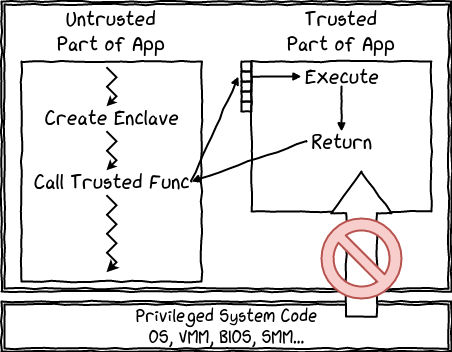
\includegraphics[scale=0.55]{Images/sgx_overview.png}
\end{frame}

\begin{frame}
    \frametitle{Overview}
    \begin{itemize}
        \visible<1->{\item Application contains own code, its own data and the enclave}
        \visible<2->{\item Enclave contains also its own code and data}
        \visible<3->{\item Enclave entry point is pre-defined during compilation}
        \visible<4->{\item SGX protects the confidentiality and integrity of the enclave code and data}
        \visible<5->{\item Enclaves can access their application memory, but not the other way arround}
        \visible<6>{\item Multi-threading is supported}
    \end{itemize}
\end{frame}

\begin{frame}
    \frametitle{Instructions}
    \begin{itemize}
        \visible<1->{\item Intel SGX defines 18 new Instructions to handle the enclaves}
        \visible<2->{\item All instructions are implemented in mircro-code, so that the behaviour can be modified}
        \visible<3> {\item 13 instructions can be used by the supervisor and 5 by normal users}
    \end{itemize}
\end{frame}

\begin{frame}
    \frametitle{Structures}
    \begin{itemize}
        \visible<1->{\item Intel SGX defines 13 new structures which are used to manage the enclave and the associated data}
        \visible<2->{\item 8 structures are used for enclave managment}
        \visible<3->{\item 3 structures are used for memory page managment}
        \visible<4>{\item 2 structures are used for resources managment}
    \end{itemize}
\end{frame}

\begin{frame}
    \frametitle{procedure application with enclave}
    \begin{columns}
        \begin{column}{0.3\textwidth}
           \begin{enumerate}
               \visible<1->{\item EENTRY instruction is executed to enter enclave}
               \visible<2->{\item The application context is saved}
               \visible<3->{\item The processor is put in enclave mode}
               \visible<4->{\item EEXIT instruction is executed to exit enclave}
               \visible<5>{\item The processor is put in normal mode}
           \end{enumerate}
        \end{column}
        \begin{column}{0.7\textwidth}
            \begin{center}
                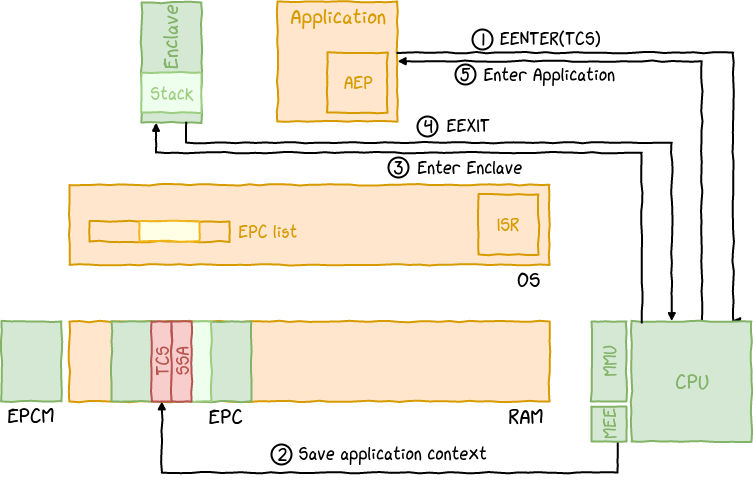
\includegraphics[scale=0.35]{Images/procedure.png}
            \end{center}
        \end{column}
        \end{columns}
\end{frame}

\begin{frame}
    \frametitle{Enclave Page Cache (EPC)}
    \begin{itemize}
        \visible<1->{\item Code and data of the enclave is stored in a special memory area, called EPC}
        \visible<2->{\item This area is encrypted by using the Memory Encryption Engine (MME)}
        \visible<3->{\item MME is an extra new and dedicated chip for Intel SGX}
        \visible<4->{\item External reads outside the chip can only observe encrypted data}
        \visible<5->{\item The pages are only decrypted when read is inside the physical processor core}
        \visible<6>{\item Keys for decrypting are generated at boot-time and are stored inside the CPU}
    \end{itemize}
\end{frame}

\begin{frame}
    \frametitle{Page Check}
    \begin{itemize}
        \visible<1->{\item Page check is extended to prevent external access to EPC}
        \visible<2->{\item The Enclave Page Cache Map (EPCM) is one of the 13 structures}
        \visible<3->{\item EPCM is used to store the pages state and contains the configuration, permissions and type of each page}
        \visible<4>{\item EPCM is also stored inside the protected memory area and grants access to the page}
    \end{itemize}
\end{frame}

\begin{frame}
    \frametitle{Page Check}
    \centering
    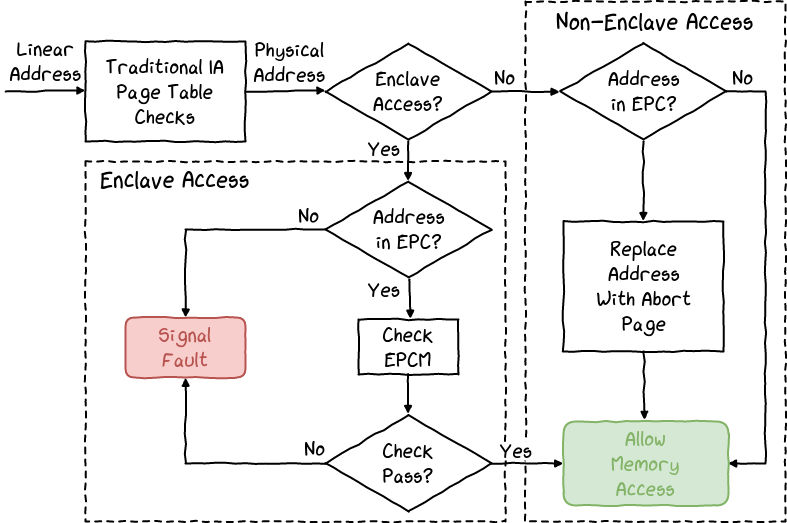
\includegraphics[scale=0.35]{Images/epc_pageCheck.png}
\end{frame}

\begin{frame}
    \frametitle{Local Attestation}
    \begin{itemize}
        \visible<1->{\item Enclaves can communicate to each other, but you have to check the local attestation}
        \visible<2->{\item Is needed to proof the other needed enclave exists}
        \visible<3->{\item The first enclave can ask the hardware to generate a credential, named report}
        \visible<4->{\item The second can verify, this resport is generated on the same platform and can now trust this enclave}
        \visible<5->{\item The second enclave has also to proof the report of the first enclave}
        \visible<6>{\item A symetric encryption is used}
    \end{itemize}
\end{frame}

\begin{frame}
    \frametitle{Remote Attestation}
    \begin{itemize}
        \visible<1->{\item }
    \end{itemize}
\end{frame}

